Here, we analyze how the phase length changes as parameters such as the model, interval size, and similarity threshold varies. The \emph{low} threshold value ($t$) is set to $t=0.1$ and the \emph{high} threshold value is set to $t=0.9$. When otherwise not noted, $t=0.1$. The computed similarity values $s$ has range $0 \leq s \leq 1.0$, where $0$ indicates intervals that are perfectly similar and $1$ indicates intervals that are not at all similar. If a computed similarity value falls below the threshold, then the tested intervals are considered similar enough to form a phase. The interval size $i$ we allow to vary between 1 and 100K. The evaluated models include instruction working sets (IWS), basic block vectors (BBV), Intel Top Down (ITD), and CPI. 

\begin{figure}[htbp]
  \begin{center}
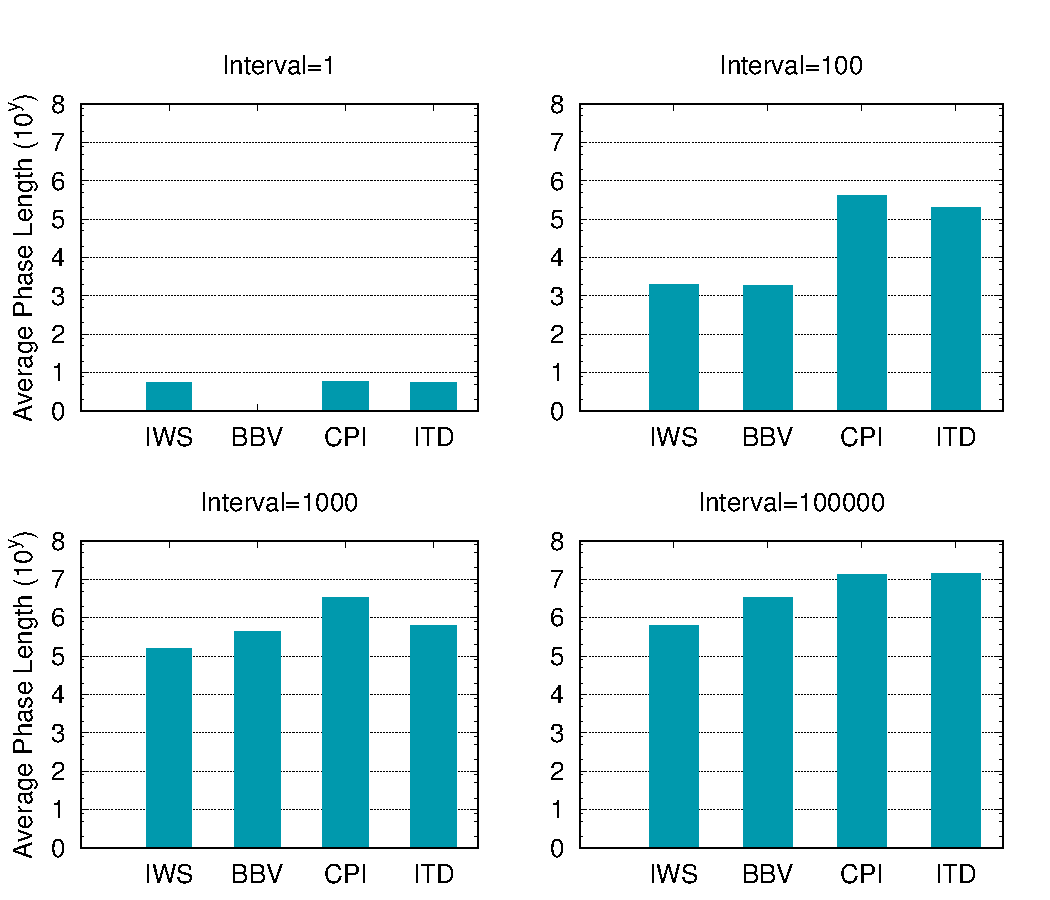
\includegraphics[width=0.99\columnwidth]{figs/phaselenavg}
  \end{center}
  \caption{At very short intervals, the phase lengths are similar across models. At longer intervals, differences in phase length begins to emerge between models.}
  \label{fig:phaselenavg}
\end{figure}

Figure~\ref{fig:phaselenavg} shows the absolute average phase length across different models and interval sizes. The range in phase length that can be observed is roughly 5-10M cycles long. The phases detected on the lower end of the size spectrum would be undetectable had the interval size been restricted to be much higher (e.g. 1M cycles). Another key observation is that the model deployed along with the interval size can have a significant effect on the phase length.  At an interval size of one cycle, we see little differences in the average phase length, which turns out to be roughly five cycles across models. As the interval size increases, we begin to see more separation with respect to the phase length across models. At an interval size of 100, both CPI and ITD have average phase lengths a couple of orders of magnitude higher then IWS and BBV. At even higher interval sizes, up to 100K, we still see some differences between models (about one order of magnitude difference). The interval size and model should be appropriately configured by the client to produce the desired phase length.

Figure~\ref{fig:phaselen} shows how the average phase length changes across the nine benchmarks as we vary all three parameters (interval size, model, and similarity threshold). One clear trend is that the phase length tends to grow as the interval size is increased. The growth rate is fast at smaller interval sizes and slows down at larger interval sizes. With respect to the similarity threshold, we see a much more pronouced growth in phase length at smaller interval sizes for higher threshold values. Along the same vein, we also generally see a much more pronounced slowdown of the growth in phase length at a higher threshold and interval size. Also note from Figure~\ref{fig:phaselen} the difference in phase length across the models. ITD tends to track more closely to CPI while IWS and BBV is tracking more closely with respect to phase length. Another interesting observation is that both CPI and ITD tend to have longer phase lengths with the former having the longest phase length, but this gap narrows given a higher threshold and interval size. To summarize, we observe the following trends with respect to phase length:

\begin{enumerate}
\item The phase length increases as the interval size increases.
\item The phase length increases at a faster rate given a higher threshold.
\item ITD tends to have a longer phase length compared to IWS and BBV and tracks more closely to CPI.
\end{enumerate}

The phase length as previously mentioned is of interest to the client in order to perform a cost benefit analysis of applying a new configuration. As Figure~\ref{fig:phaselen} shows, all three parameters (interval size, model, and similarity threshold) can impact the phase length and can be tweaked by the client in order to obtain the desired length. If a client desires a longer phase length, then that can be accomplished by increasing the interval size, relaxing the threshold, or switching models. The design of a phase analysis framework should enable the client to easily adjust these parameters to achieve the desired phase length. 


\begin{figure}[htbp]
  \begin{center}
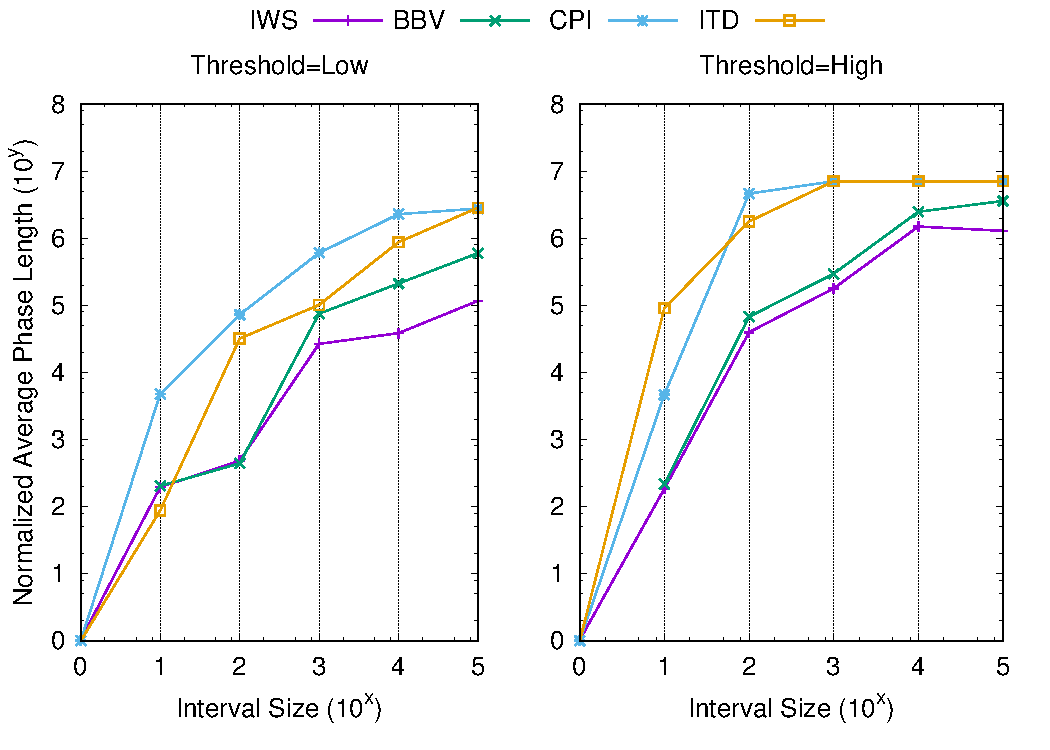
\includegraphics[width=0.99\columnwidth]{figs/phaselenfixthreshold}
  \end{center}
  \caption{All three parameters (interval size, model, and threshold) appear to have a significant effect on the phase length.}
  \label{fig:phaselen}
\end{figure}


